

\chapter{贾夫人仙逝扬州城\hspace{.5em}冷子兴演说荣国府}
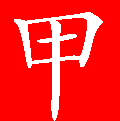
\includegraphics[width=3mm]{../Images/00002}{\kaishu 此回亦非正文,本旨只在冷子兴一人,即俗谓``冷中出热,无中生有''也。其演说荣府一篇者,盖因族大人多,若从作者笔下一一叙出,尽一二回不能得明,则成何文字?故借用冷子一人,略出其大半,使阅者心中,已有一荣府隐隐在心,然后用黛玉、宝钗等两三次皴染,则耀然于心中眼中矣。此即画家三染法也。


未写荣府正人,先写外戚,是由远及近、由小至大也。若使先叙出荣府,然后一一叙及外戚,又一一至朋友、至奴仆,其死板拮据之笔,岂作``十二钗''人手中之物也?今先写外戚者,正是写荣国一府也。故又怕闲文赘累,开笔即写贾夫人已死,是特使黛玉入荣之速也。通灵宝玉于士隐梦中一出,今于子兴口中一出,阅者已洞然矣。然后于黛玉、宝钗二人目中极精极细一描,则是文章锁合处。盖不肯一笔直下,有若放闸之水、燃信之爆,使其精华一泄而无馀也。究竟此玉原应出自钗、黛目中,方有照应。今预从子兴口中说出,实虽写而却未写。观其后文可知。此一回{[}文{]}则是虚敲傍击之文,笔则是反逆隐回之笔。

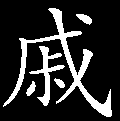
\includegraphics[width=3mm]{../Images/00005}  \kaishu 以百回之大文,先以此回作两大笔以冒之,诚是大观。世态人情,尽盘旋于其间,而一丝不乱,非具龙象力者,其孰能哉?}

诗云:{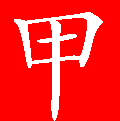
\includegraphics[width=3mm]{../Images/00002}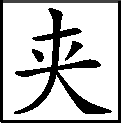
\includegraphics[width=3mm]{../Images/00012}\footnotesize \kaishu 只此一诗便妙极!此等才情,自是雪芹平生所长,余自谓评书,非关评诗也。}

一局输赢料不真,香销茶尽尚逡巡。

欲知目下兴衰兆,须问旁观冷眼人。{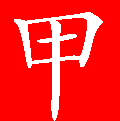
\includegraphics[width=3mm]{../Images/00002}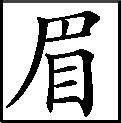
\includegraphics[width=3mm]{../Images/00010}\footnotesize \kaishu 故用冷子兴演说。}

却说封肃因听见公差传唤,忙出来陪笑启问。那些人只嚷:``快请出甄爷来!''{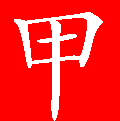
\includegraphics[width=3mm]{../Images/00002}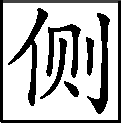
\includegraphics[width=3mm]{../Images/00011}\footnotesize \kaishu 一丝不乱。}封肃忙陪笑道:``小人姓封,并不姓甄。只有当日小婿姓甄,今已出家一二年了,不知可是问他?''那些公人道:``我们也不知什么`真'`假',{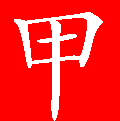
\includegraphics[width=3mm]{../Images/00002}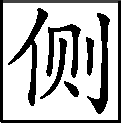
\includegraphics[width=3mm]{../Images/00011}\footnotesize \kaishu 点睛妙笔。}因奉太爷之命来问。他既是你女婿,便带了你去亲见太爷面禀,省得乱跑。''说着,不容封肃多言,大家推拥他去了。封家人各各惊慌,不知何兆。

那天约有二更时分,只见封肃方回来,欢天喜地。{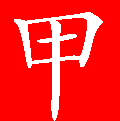
\includegraphics[width=3mm]{../Images/00002}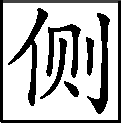
\includegraphics[width=3mm]{../Images/00011}\footnotesize \kaishu 出自封肃口内,便省却多少闲文。}众人忙问端的。他乃说道:``原来本府新升的太爷,姓贾名化,本胡州人氏,曾与女婿旧日相交。{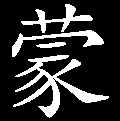
\includegraphics[width=3mm]{../Images/00006}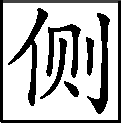
\includegraphics[width=3mm]{../Images/00011}\footnotesize \kaishu 世态精神,叠露于数语间。}方才在咱门前过去,因看见娇杏{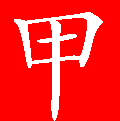
\includegraphics[width=3mm]{../Images/00002}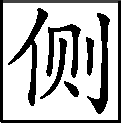
\includegraphics[width=3mm]{../Images/00011}\footnotesize \kaishu 侥幸也。◇托言当日丫头回顾,故有今日,亦不过偶然侥幸耳,非真实得尘中英杰也。非近日小说中满纸红拂紫烟之可比。 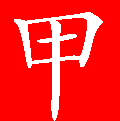
\includegraphics[width=3mm]{../Images/00002}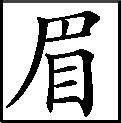
\includegraphics[width=3mm]{../Images/00010}\footnotesize \kaishu 余批重出。余阅此书,偶有所得,即笔录之。非从首至尾阅过复从首加批者,故偶有复处。且诸公之批,自是诸公眼界;脂斋之批,亦有脂斋取乐处。后每一阅,亦必有一语半言,重加批评于侧,故又有于前后照应之说等批。}那丫头买线,所以他只当女婿移住于此。我一一将原故回明,那太爷倒伤感叹息了一回。又问外孙女儿,{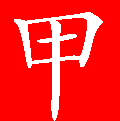
\includegraphics[width=3mm]{../Images/00002}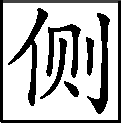
\includegraphics[width=3mm]{../Images/00011}\footnotesize \kaishu 细。}我说看灯丢了。太爷说:`不妨,我自使番役务必采访回来。'{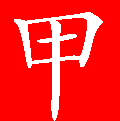
\includegraphics[width=3mm]{../Images/00002}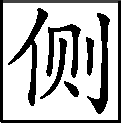
\includegraphics[width=3mm]{../Images/00011}\footnotesize \kaishu 为葫芦案伏线。}说了一回话,临走倒送了我二两银子。''{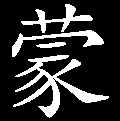
\includegraphics[width=3mm]{../Images/00006}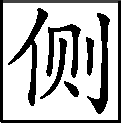
\includegraphics[width=3mm]{../Images/00011}\footnotesize \kaishu 此事最要紧。}甄家娘子听了,不免心中伤感。{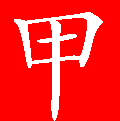
\includegraphics[width=3mm]{../Images/00002}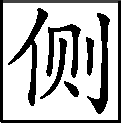
\includegraphics[width=3mm]{../Images/00011}\footnotesize \kaishu 所谓``旧事凄凉不可闻''也。}一宿无话。

至次日,早有雨村遣人送两封银子、四匹锦缎,答谢甄家娘子,{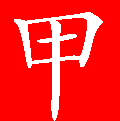
\includegraphics[width=3mm]{../Images/00002}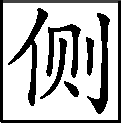
\includegraphics[width=3mm]{../Images/00011}\footnotesize \kaishu 雨村已是下流人物,看此,今之如雨村者亦未有矣。}又寄一封密书与封肃,转托他向甄家娘子要那娇杏作二房。{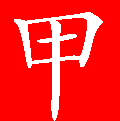
\includegraphics[width=3mm]{../Images/00002}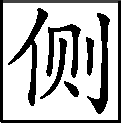
\includegraphics[width=3mm]{../Images/00011}\footnotesize \kaishu 谢礼却为此。险哉,人之心也!}封肃喜得屁滚尿流,巴不得去奉承,便在女儿前一力撺掇成了,{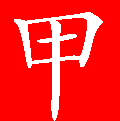
\includegraphics[width=3mm]{../Images/00002}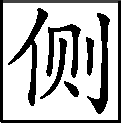
\includegraphics[width=3mm]{../Images/00011}\footnotesize \kaishu 一语道尽。}乘夜只用一乘小轿,便把娇杏送进去了。雨村欢喜自不必说。{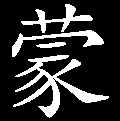
\includegraphics[width=3mm]{../Images/00006}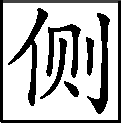
\includegraphics[width=3mm]{../Images/00011}\footnotesize \kaishu 知己相逢,得遂平生,一大快事。}乃封百金赠封肃,外又谢甄家娘子许多物事,令其好生养赡,以待寻访女儿下落。{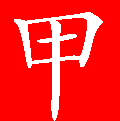
\includegraphics[width=3mm]{../Images/00002}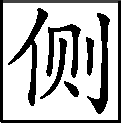
\includegraphics[width=3mm]{../Images/00011}\footnotesize \kaishu 找前伏后。}封肃回家无话。{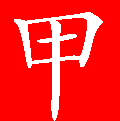
\includegraphics[width=3mm]{../Images/00002}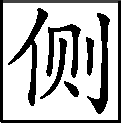
\includegraphics[width=3mm]{../Images/00011}\footnotesize \kaishu 士隐家一段小荣枯至此结住,所谓``真不去,假焉来''也!}

却说娇杏这丫鬟,便是那年回顾雨村者。因偶然一顾,便弄出这段事来,亦是自己意料不到之奇缘。{{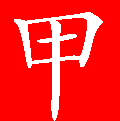
\includegraphics[width=3mm]{../Images/00002}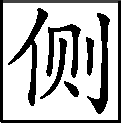
\includegraphics[width=3mm]{../Images/00011}\footnotesize \kaishu 注明一笔,更妥当。 }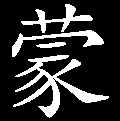
\includegraphics[width=3mm]{../Images/00006}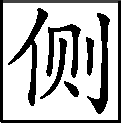
\includegraphics[width=3mm]{../Images/00011}\footnotesize \kaishu 点出情事。}谁想他命运两济,{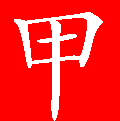
\includegraphics[width=3mm]{../Images/00002}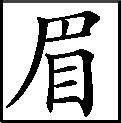
\includegraphics[width=3mm]{../Images/00010}\footnotesize \kaishu 好极!与英莲``有命无运''四字遥遥相映射。莲,主也;杏,仆也。今莲反无运,而杏则两全,可知世人原在运数,不在眼下之高低也。此则大有深意存焉。}不承望自到雨村身边,只一年便生了一子,又半载,雨村嫡妻忽染疾下世,雨村便将他扶册作正室夫人了。正是:

偶因一着错,{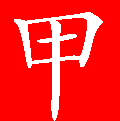
\includegraphics[width=3mm]{../Images/00002}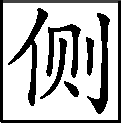
\includegraphics[width=3mm]{../Images/00011}\footnotesize \kaishu 妙极!盖女儿原不应私顾外人之谓。}

便为人上人。{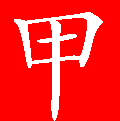
\includegraphics[width=3mm]{../Images/00002}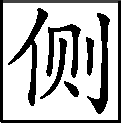
\includegraphics[width=3mm]{../Images/00011}\footnotesize \kaishu 更妙!可知守礼俟命者终为饿莩。其调侃寓意不小。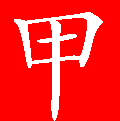
\includegraphics[width=3mm]{../Images/00002}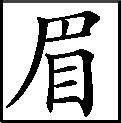
\includegraphics[width=3mm]{../Images/00010}\footnotesize \kaishu 从来只见集古、集唐等句,未见集俗语者。此又更奇之至!}

原来,雨村因那年士隐赠银之后,他于十六日便起身入都。至大比之期,不料他十分得意,已会了进士,选入外班,今已升了本府知府。虽才干优长,未免有些贪酷之弊,且又恃才侮上,那些官员皆侧目而视。{\includegraphics[width=3mm]{../Images/00002}\includegraphics[width=3mm]{../Images/00011}\footnotesize \kaishu 此亦奸雄必有之理。}不上一年,便被上司寻了个空隙,作成一本,参他``生情狡猾,擅纂礼仪,且沽清正之名,而暗结虎狼之属,致使地方多事,民命不堪''{\includegraphics[width=3mm]{../Images/00002}\includegraphics[width=3mm]{../Images/00011}\footnotesize \kaishu 此亦奸雄必有之事。}等语。龙颜大怒,即批革职。{\includegraphics[width=3mm]{../Images/00006}\includegraphics[width=3mm]{../Images/00011}\footnotesize \kaishu 罪重而法轻,何其幸也。}该部文书一到,本府官员无不喜悦。那雨村心中虽十分惭恨,却面上全无一点怨色,仍是喜悦自若。{\includegraphics[width=3mm]{../Images/00002}\includegraphics[width=3mm]{../Images/00011}\footnotesize \kaishu 此亦奸雄必有之态。}交代过公事,将历年做官积的些资本并家小人属送至原籍,安排妥协,{\includegraphics[width=3mm]{../Images/00002}\includegraphics[width=3mm]{../Images/00011}\footnotesize \kaishu 先云``根基已尽'',故今用此四字,细甚!}却又自己担风袖月,游览天下胜迹。{\includegraphics[width=3mm]{../Images/00002}\includegraphics[width=3mm]{../Images/00011}\footnotesize \kaishu 已伏下至金陵一节矣。}

那日,偶又游至维扬地面,因闻得今岁鹾政点的是林如海。这林如海姓林名海,表字如海。{\includegraphics[width=3mm]{../Images/00002}\includegraphics[width=3mm]{../Images/00011}\footnotesize \kaishu 盖云``学海文林''也。总是暗写黛玉。}乃是前科的探花,今已升至兰台寺大夫,{\includegraphics[width=3mm]{../Images/00002}\includegraphics[width=3mm]{../Images/00010}\footnotesize \kaishu 官制半遵古名亦好。余最喜此等半有半无,半古半今,事之所无,理之必有,极玄极幻,荒唐不经之处。}本贯姑苏{\includegraphics[width=3mm]{../Images/00002}\includegraphics[width=3mm]{../Images/00011}\footnotesize \kaishu 十二钗正出之地,故用真。}人氏,今钦点出为巡盐御史,到任方一月有馀。

原来这林如海之祖,曾袭过列侯,今到如海,业经五世。起初时,只封袭三世,因当今隆恩盛德,远迈前代,{\includegraphics[width=3mm]{../Images/00002}\includegraphics[width=3mm]{../Images/00010}\footnotesize \kaishu 可笑近时小说中,无故极力称扬浪子淫女,临收结时,还必致感动朝廷,使君父同入其情欲之界,明遂其意,何无人心之至!不知彼作者有何好处,有何谢报到朝廷廊庙之上,直将半生淫朽,秽渎睿聪,又苦拉君父作一干证护身符,强媒硬保,得遂其淫欲哉!}额外加恩,至如海之父,又袭了一代;至如海,便从科第出身。虽系钟鼎之家,却亦是书香{\includegraphics[width=3mm]{../Images/00002}\includegraphics[width=3mm]{../Images/00011}\footnotesize \kaishu 要紧二字,盖钟鼎亦必有书香方至美。}之族。只可惜这林家支庶不盛,子孙有限,虽有几门,却与如海俱是堂族而已,没甚亲支嫡派的。{\includegraphics[width=3mm]{../Images/00002}\includegraphics[width=3mm]{../Images/00011}\footnotesize \kaishu 总为黛玉极力一写。}今如海年已四十,只有一个三岁之子,偏又于去岁死了。虽有几房姬妾,{\includegraphics[width=3mm]{../Images/00002}\includegraphics[width=3mm]{../Images/00011}\footnotesize \kaishu 带写贤妻。}奈他命中无子,亦无可如何之事。今只有嫡妻贾氏,生得一女,乳名黛玉,{\includegraphics[width=3mm]{../Images/00006}\includegraphics[width=3mm]{../Images/00011}\footnotesize \kaishu 绛珠初见。}年方五岁。夫妻无子,故爱女如珍,且又见他聪明清秀,{\includegraphics[width=3mm]{../Images/00002}\includegraphics[width=3mm]{../Images/00011}\footnotesize \kaishu 看他写黛玉,只用此四字。可笑近来小说中,满纸``天下无二''``古今无双''等字。}便也欲使他读书识得几个字,不过假充养子之意,聊解膝下荒凉之叹。{\includegraphics[width=3mm]{../Images/00002}\includegraphics[width=3mm]{../Images/00010}\footnotesize \kaishu 如此叙法,方是至情至理之妙文。最可笑者,近小说中满纸班昭蔡琰、文君道韫。}

雨村正值偶感风寒,病在旅店,将一月光景方渐愈。一因身体劳倦,二因盘费不继,也正欲寻个合式之处,暂且歇下。幸有两个旧友,亦在此境居住,{\includegraphics[width=3mm]{../Images/00002}\includegraphics[width=3mm]{../Images/00011}\footnotesize \kaishu 写雨村自得意后之交识也。◇又为冷子兴作引。}因闻得鹾政欲聘一西宾,雨村便相托友力,谋了进去,且作安身之计。妙在只一个女学生,并两个伴读丫鬟,这女学生年又极小,身体又极怯弱,工课不限多寡,故十分省力。

堪堪又是一载的光阴,谁知女学生之母贾氏夫人一疾而终。女学生侍汤奉药,守丧尽哀,{\includegraphics[width=3mm]{../Images/00006}\includegraphics[width=3mm]{../Images/00011}\footnotesize \kaishu 先要使黛玉哭起。}遂又将要辞馆别图。林如海意欲令女守制读书,故又将他留下。近因女学生哀痛过伤,本自怯弱多病的,{\includegraphics[width=3mm]{../Images/00002}\includegraphics[width=3mm]{../Images/00011}\footnotesize \kaishu 又一染。}触犯旧症,遂连日不曾上学。{\includegraphics[width=3mm]{../Images/00002}\includegraphics[width=3mm]{../Images/00010}\footnotesize \kaishu 上半回已终,写``仙逝''正为黛玉也。故一句带过,恐闲文有妨正笔。}

雨村闲居无聊,每当风日晴和,饭后便出来闲步。这日,偶至郭外,意欲赏鉴那村野风光。{\includegraphics[width=3mm]{../Images/00002}\includegraphics[width=3mm]{../Images/00010}\footnotesize \kaishu 大都世人意料此,终不能此;不及彼者,而反及彼。故特书意在村野风光,却忽遇见子兴,一篇荣国繁华气象。}忽信步至一山环水旋、茂林深竹之处,隐隐有座庙宇,门巷倾颓,墙垣朽败,门前有额,题着``智通寺''三字,{\includegraphics[width=3mm]{../Images/00002}\includegraphics[width=3mm]{../Images/00011}\footnotesize \kaishu 谁为智者?又谁能通?一叹。}门旁又有一副旧破的对联,曰:

身后有馀忘缩手,眼前无路想回头。{\includegraphics[width=3mm]{../Images/00002}\includegraphics[width=3mm]{../Images/00012}\footnotesize \kaishu 先为宁、荣诸人当头一喝,却是为余一喝。}

雨村看了,因想到:``这两句话,文虽浅,其意则深。{\includegraphics[width=3mm]{../Images/00002}\includegraphics[width=3mm]{../Images/00011}\footnotesize \kaishu 一部书之总批。}也曾游过些名山大刹,倒不曾见过这话头,其中想必有个翻过筋斗来的亦未可知,{\includegraphics[width=3mm]{../Images/00002}\includegraphics[width=3mm]{../Images/00011}\footnotesize \kaishu 随笔带出禅机,又为后文多少语录不落空。}何不进去试试?''想着,走入看时,只有一个聋肿\href{../Text/part0006_split_000.html\#lnkback_1_a}{\textsuperscript{①}}老僧在那里煮粥。{\includegraphics[width=3mm]{../Images/00002}\includegraphics[width=3mm]{../Images/00011}\footnotesize \kaishu 是雨村火气。}雨村见了,便不在意。{\includegraphics[width=3mm]{../Images/00002}\includegraphics[width=3mm]{../Images/00011}\footnotesize \kaishu 火气。}及至问他两句话,那老僧既聋且昏,{{\includegraphics[width=3mm]{../Images/00002}\includegraphics[width=3mm]{../Images/00011}\footnotesize \kaishu 是翻过来的。 }\includegraphics[width=3mm]{../Images/00006}\includegraphics[width=3mm]{../Images/00011}\footnotesize \kaishu 欲写冷子兴,偏闲闲有许多着力语。}齿落舌钝,{\includegraphics[width=3mm]{../Images/00002}\includegraphics[width=3mm]{../Images/00011}\footnotesize \kaishu 是翻过来的。}所答非所问。

雨村不耐烦,便仍出来,{\includegraphics[width=3mm]{../Images/00002}\includegraphics[width=3mm]{../Images/00010}\footnotesize \kaishu 毕竟雨村还是俗眼,只能识得阿凤、宝玉、黛玉等未觉之先,却不识得既证之后。◇未出宁、荣繁华盛处,却先写一荒凉小境;未写通部入世迷人,却先写一出世醒人。回风舞雪,倒峡逆波,别小说中所无之法。}意欲到那村肆中沽酒三杯,以助野趣。于是款步行来,刚入肆门,只见座上吃酒之客有一人起身大笑,接了出来,口内说:``奇遇,奇遇!''雨村忙看时,此人是都中古董行中贸易的号冷子兴者,{\includegraphics[width=3mm]{../Images/00002}\includegraphics[width=3mm]{../Images/00011}\footnotesize \kaishu 此人不过借为引绳,不必细写。}旧日在都相识。雨村最赞这冷子兴是个有作为大本领的人,{\includegraphics[width=3mm]{../Images/00005}\includegraphics[width=3mm]{../Images/00012}\footnotesize \kaishu 不赞出则文不灵活,而冷子兴之谈吐似觉唐突矣。}这子兴又借雨村斯文之名,故二人说话投机,最相契合。雨村忙亦笑问:``老兄何日到此?弟竟不知。今日偶遇,真奇缘也。''子兴道:``去年岁底到家,今因还要入都,从此顺路找个敝友说一句话,承他之情,留我多住两日。我也无甚紧事,且盘桓两日,待月半时也就起身了。今日敝友有事,我因闲步至此,且歇歇脚。不期这样巧遇!''一面说,一面让雨村同席坐了,另整上酒肴来。二人闲谈慢饮,叙些别后之事。{{\includegraphics[width=3mm]{../Images/00002}\includegraphics[width=3mm]{../Images/00011}\footnotesize \kaishu 好!若多谈则累赘。 }\includegraphics[width=3mm]{../Images/00006}\includegraphics[width=3mm]{../Images/00011}\footnotesize \kaishu 又抛一笔。}

雨村因问:``近日都中可有新闻没有?''{\includegraphics[width=3mm]{../Images/00002}\includegraphics[width=3mm]{../Images/00011}\footnotesize \kaishu 不突然,亦常问常答之言。}子兴道:``倒没有什么新闻,倒是老先生你贵同宗家,{\includegraphics[width=3mm]{../Images/00002}\includegraphics[width=3mm]{../Images/00011}\footnotesize \kaishu 雨村已无族中矣,何及此耶?看他下文。}出了一件小小的异事。''雨村笑道:``弟族中无人在都,何谈及此?''子兴笑道:``你们同姓,岂非同宗一族?''雨村问是谁家。

子兴道:``荣国府贾府中,可也不玷辱了先生的门楣了?''{\includegraphics[width=3mm]{../Images/00002}\includegraphics[width=3mm]{../Images/00011}\footnotesize \kaishu 刳小人之心肺,闻小人之口角。}雨村笑道:``原来是他家。若论起来,寒族人丁却不少,自东汉贾复以来,支派繁盛,各省皆有,{{\includegraphics[width=3mm]{../Images/00002}\includegraphics[width=3mm]{../Images/00011}\footnotesize \kaishu 此话纵真,亦必谓是雨村欺人语。 }\includegraphics[width=3mm]{../Images/00006}\includegraphics[width=3mm]{../Images/00011}\footnotesize \kaishu 如闻其声。}谁能逐细考查?若论荣国一支,却是同谱。但他那等荣耀,我们不便去攀扯,至今越发生疏难认了。''子兴叹{\includegraphics[width=3mm]{../Images/00002}\includegraphics[width=3mm]{../Images/00011}\footnotesize \kaishu 叹得怪。}道:``老先生休如此说。如今这荣国两门,也都萧疏了,不比先时的光景。''{\includegraphics[width=3mm]{../Images/00002}\includegraphics[width=3mm]{../Images/00011}\footnotesize \kaishu 记清此句。可知书中之荣府已是末世了。}雨村道:``当日宁荣两宅的人口极多,如何就萧疏了?''{\includegraphics[width=3mm]{../Images/00002}\includegraphics[width=3mm]{../Images/00011}\footnotesize \kaishu 作者之意原只写末世,此已是贾府之末世了。}冷子兴道:``正是,说来也话长。''雨村道:``去岁我到金陵地界,因欲游览六朝遗迹,那日进了石头城,{\includegraphics[width=3mm]{../Images/00002}\includegraphics[width=3mm]{../Images/00011}\footnotesize \kaishu 点睛,神妙。}从他老宅门前经过。街东是宁国府,街西是荣国府,二宅相连,竟将大半条街占了。大门前虽冷落无人,{\includegraphics[width=3mm]{../Images/00002}\includegraphics[width=3mm]{../Images/00011}\footnotesize \kaishu 好!写出空宅。}隔着围墙一望,里面厅殿楼阁,也还都峥嵘轩峻,就是后{\includegraphics[width=3mm]{../Images/00002}\includegraphics[width=3mm]{../Images/00011}\footnotesize \kaishu ``后''字何不直用``西''字?◇恐先生堕泪,故不敢用``西''字。}一带花园子里,树木山石,也还都有蓊蔚洇润之气,那里像个衰败之家?''

冷子兴笑道:``亏你是进士出身,原来不通!古人有云:`百足之虫,死而不僵。'如今虽说不及先年那样兴盛,较之平常仕宦之家,到底气象不同。如今生齿日繁,事务日盛,主仆上下,安富尊荣者尽多,运筹谋画者无一,{\includegraphics[width=3mm]{../Images/00002}\includegraphics[width=3mm]{../Images/00011}\footnotesize \kaishu 二语乃今古富贵世家之大病。}其日用排场费用,又不能将就省俭,如今外面的架子虽未甚倒,{\includegraphics[width=3mm]{../Images/00002}\includegraphics[width=3mm]{../Images/00011}\footnotesize \kaishu ``甚''字好!盖已半倒矣。}内囊却也尽上来了。{\includegraphics[width=3mm]{../Images/00006}\includegraphics[width=3mm]{../Images/00011}\footnotesize \kaishu 世家兴败,寄口与人,诚可悲夫。}这还是小事,更有一件大事:谁知这样钟鸣鼎食之家,翰墨诗书之族,{\includegraphics[width=3mm]{../Images/00002}\includegraphics[width=3mm]{../Images/00011}\footnotesize \kaishu 两句写出荣府。}如今的儿孙,竟一代不如一代了!''{\includegraphics[width=3mm]{../Images/00002}\includegraphics[width=3mm]{../Images/00010}\footnotesize \kaishu 文是极好之文,理是必有之理,话则极痛极悲之话。}雨村听说,也纳罕道:``这样诗书之家,岂有不善教育之理?别家不知,只说这宁、荣二宅,是最教子有方的。''{\includegraphics[width=3mm]{../Images/00002}\includegraphics[width=3mm]{../Images/00011}\footnotesize \kaishu 一转有力。}

子兴叹道:``正说的是这两门呢。待我告诉你。当日宁国公{\includegraphics[width=3mm]{../Images/00002}\includegraphics[width=3mm]{../Images/00011}\footnotesize \kaishu 演。}与荣国公{\includegraphics[width=3mm]{../Images/00002}\includegraphics[width=3mm]{../Images/00011}\footnotesize \kaishu 源。}是一母同胞弟兄两个。宁公居长,生了四个儿子。{\includegraphics[width=3mm]{../Images/00002}\includegraphics[width=3mm]{../Images/00011}\footnotesize \kaishu 贾蔷、贾菌之祖,不言可知矣。}宁公死后,长子贾代化袭了官,{\includegraphics[width=3mm]{../Images/00002}\includegraphics[width=3mm]{../Images/00011}\footnotesize \kaishu 第二代。}也养了两个儿子。长名贾敷,至八九岁上便死了,只剩了次子贾敬袭了官,{\includegraphics[width=3mm]{../Images/00002}\includegraphics[width=3mm]{../Images/00011}\footnotesize \kaishu 第三代。}如今一味好道,只爱烧丹炼汞,{{\includegraphics[width=3mm]{../Images/00002}\includegraphics[width=3mm]{../Images/00011}\footnotesize \kaishu 亦是大族末世常有之事。叹叹! }\includegraphics[width=3mm]{../Images/00006}\includegraphics[width=3mm]{../Images/00011}\footnotesize \kaishu 偏先从好神仙的苦处说来。}馀者一概不在心上。幸而早年留下一子,名唤贾珍,{\includegraphics[width=3mm]{../Images/00002}\includegraphics[width=3mm]{../Images/00011}\footnotesize \kaishu 第四代。}因他父亲一心想作神仙,把官倒让他袭了。他父亲又不肯回原籍来,只在都中城外和道士们胡羼。这位珍爷也倒生了一个儿子,今年才十六岁,名叫贾蓉。{\includegraphics[width=3mm]{../Images/00002}\includegraphics[width=3mm]{../Images/00011}\footnotesize \kaishu 至蓉五代。}如今敬老爹一概不管。这珍爷那肯读书,只是一味高乐不已,把宁国府竟翻了过来,也没有人敢来管他。{\includegraphics[width=3mm]{../Images/00002}\includegraphics[width=3mm]{../Images/00011}\footnotesize \kaishu 伏后文。}再说荣府你听,方才所说异事,就出在这里。自荣公死后,长子贾代善袭了官,{\includegraphics[width=3mm]{../Images/00002}\includegraphics[width=3mm]{../Images/00011}\footnotesize \kaishu 第二代。}娶的金陵世勋史侯家的小姐{\includegraphics[width=3mm]{../Images/00002}\includegraphics[width=3mm]{../Images/00011}\footnotesize \kaishu 因湘云,故及之。}为妻,生了两个儿子:长子贾赦,次子贾政。{\includegraphics[width=3mm]{../Images/00002}\includegraphics[width=3mm]{../Images/00011}\footnotesize \kaishu 第三代。}如今代善早已去世,太夫人{\includegraphics[width=3mm]{../Images/00002}\includegraphics[width=3mm]{../Images/00011}\footnotesize \kaishu 记真,湘云祖姑史氏太君也。}尚在。长子贾赦袭着官。次子贾政,自幼酷喜读书,祖父最疼。原欲以科甲出身的,不料代善临终时遗本一上,皇上因恤先臣,即时令长子袭官外,问还有几子,立刻引见,遂额外赐了这政老爹一个主事之衔,{\includegraphics[width=3mm]{../Images/00002}\includegraphics[width=3mm]{../Images/00011}\footnotesize \kaishu 嫡真实事,}\href{../Text/part0006_split_000.html\#lnkback_2_a}{\textsuperscript{②}}{非妄拟也。}令其入部习学,如今现已升了员外郎了。{\includegraphics[width=3mm]{../Images/00002}\includegraphics[width=3mm]{../Images/00011}\footnotesize \kaishu 总是称功颂德。}这政老爹的夫人王氏,{\includegraphics[width=3mm]{../Images/00002}\includegraphics[width=3mm]{../Images/00011}\footnotesize \kaishu 记清。}头胎生的公子,名唤贾珠,十四岁进学,不到二十岁就娶了妻生了子,{\includegraphics[width=3mm]{../Images/00002}\includegraphics[width=3mm]{../Images/00011}\footnotesize \kaishu 此即贾兰也。至兰第五代。}一病死了。{\includegraphics[width=3mm]{../Images/00002}\includegraphics[width=3mm]{../Images/00010}\footnotesize \kaishu 略可望者即死,叹叹!}第二胎生了一位小姐,生在大年初一,这就奇了;不想次年\href{../Text/part0006_split_000.html\#lnkback_3_a}{\textsuperscript{③}}又生了一位公子,{\includegraphics[width=3mm]{../Images/00002}\includegraphics[width=3mm]{../Images/00010}\footnotesize \kaishu 一部书中第一人却如此淡淡带出,故不见后来玉兄文字繁难。}说来更奇:一落胎胞,嘴里便衔下一块五彩晶莹的玉来,上面还有许多字迹,{\includegraphics[width=3mm]{../Images/00002}\includegraphics[width=3mm]{../Images/00011}\footnotesize \kaishu 青埂顽石已得下落。}就取名叫作宝玉。你道是新奇异事不是?''{\includegraphics[width=3mm]{../Images/00009}\includegraphics[width=3mm]{../Images/00012}\footnotesize \kaishu 正是宁、荣二处支谱。}

雨村笑道:``果然奇异。只怕这人来历不小。''子兴冷笑道:``万人皆如此说,因而乃祖母便先爱如珍宝。那年周岁时,政老爹便要试他将来的志向,便将那世上所有之物摆了无数,与他抓取。谁知他一概不取,伸手只把些脂粉钗环抓来。政老爹便大怒了,说:`将来酒色之徒耳!'因此便大不喜悦。独那史老太君还是命根一样。说来又奇,如今长了七八岁,虽然淘气异常,但其聪明乖觉处,百个不及他一个。说起孩子话来也奇怪,他说:`女儿是水作的骨肉,男人是泥作的骨肉。{\includegraphics[width=3mm]{../Images/00002}\includegraphics[width=3mm]{../Images/00011}\footnotesize \kaishu 真千古奇文奇情。}我见了女儿,我便清爽;见了男人,便觉浊臭逼人。'你道好笑不好笑?将来色鬼无疑了!''{\includegraphics[width=3mm]{../Images/00002}\includegraphics[width=3mm]{../Images/00011}\footnotesize \kaishu 没有这一句,雨村如何罕然厉色,并后奇奇怪怪之论?}雨村罕然厉色忙止道:``非也!可惜你们不知道这人来历。大约政老前辈也错以淫魔色鬼看待了。若非多读书识事,加以致知格物之功,悟道参玄之力者,不能知也。''

子兴见他说得这样重大,忙请教其端。雨村道:``天地生人,除大仁大恶两种,馀者皆无大异。若大仁者,则应运而生,大恶者,则应劫而生。运生世治,劫生世危。尧、舜、禹、汤、文、武、周、召、孔、孟、董、韩、周、程、张、朱,皆应运而生者。蚩尤、共工、桀、纣、始皇、王莽、曹操、桓温、安禄山、秦桧等,皆应劫而生者。{\includegraphics[width=3mm]{../Images/00002}\includegraphics[width=3mm]{../Images/00011}\footnotesize \kaishu 此亦略举大概几人而言。}大仁者,修治天下;大恶者,挠乱天下。清明灵秀,天地之正气,仁者之所秉也;残忍乖僻,天地之邪气,恶者之所秉也。今当运隆祚永之朝,太平无为之世,清明灵秀之气所秉者,上至朝廷,下至草野,比比皆是。所馀之秀气,漫无所归,遂为甘露,为和风,洽然溉及四海。彼残忍乖僻之邪气,不能荡溢于光天化日之中,遂凝结充塞于深沟大壑之内,偶因风荡,或被云摧,略有摇动感发之意,一丝半缕误而泄出者,偶值灵秀之气适过,正不容邪,邪复妒正,{\includegraphics[width=3mm]{../Images/00002}\includegraphics[width=3mm]{../Images/00011}\footnotesize \kaishu 譬得好。}两不相下,亦如风水雷电,地中既遇,既不能消,又不能让,必至搏击掀发后始尽。故其气亦必赋人,发泄一尽始散。使男女偶秉此气而生者,在上则不能成仁人君子,下亦不能为大凶大恶。{\includegraphics[width=3mm]{../Images/00002}\includegraphics[width=3mm]{../Images/00011}\footnotesize \kaishu 恰极,是确论。}置之于万万人中,其聪俊灵秀之气,则在万万人之上,其乖僻邪谬、不近人情之态,又在万万人之下。若生于公侯富贵之家,则为情痴情种,若生于诗书清贫之族,则为逸士高人,{\includegraphics[width=3mm]{../Images/00006}\includegraphics[width=3mm]{../Images/00011}\footnotesize \kaishu 巧笔奇言,另开{[}生{]}面。但此数语,恐误尽聪明后生者。}纵再偶生于薄祚寒门,断不能为走卒健仆,甘遭庸人驱制驾驭,必为奇优名倡。如前代之许由、陶潜、阮籍、嵇康、刘伶、王谢二族、顾虎头、陈后主、唐明皇、宋徽宗、刘庭芝、温飞卿、米南宫、石曼卿、柳耆卿、秦少游,近日之倪云林、唐伯虎、祝枝山,再如李龟年、黄幡绰、敬新磨、卓文君、红拂、薛涛、崔莺、朝云之流。此皆易地则同之人也。''

子兴道:``依你说,`成则王侯败则贼'{\includegraphics[width=3mm]{../Images/00002}\includegraphics[width=3mm]{../Images/00011}\footnotesize \kaishu 《女仙外史》中论魔道已奇,此又非《外史》之立意,故觉愈奇。}了。''雨村道:``正是这意。你还不知,我自革职以来,这两年遍游名省,也曾遇见两个异样孩子。{\includegraphics[width=3mm]{../Images/00002}\includegraphics[width=3mm]{../Images/00011}\footnotesize \kaishu 先虚陪一个。}所以,方才你一说这宝玉,我就猜着了八九亦是这一派人物。不用远说,只金陵城内,钦差金陵省体仁院总裁{\includegraphics[width=3mm]{../Images/00002}\includegraphics[width=3mm]{../Images/00011}\footnotesize \kaishu 此衔无考,亦因寓怀而设,置而勿论。}甄家,{\includegraphics[width=3mm]{../Images/00002}\includegraphics[width=3mm]{../Images/00010}\footnotesize \kaishu 又一个真正之家,特与假家遥对,故写假则知真。}你可知么?''子兴道:``谁人不知!这甄府和贾府就是老亲,又系世交。两家来往,极其亲热的。便在下也和他家来往非止一日了。''{\includegraphics[width=3mm]{../Images/00002}\includegraphics[width=3mm]{../Images/00011}\footnotesize \kaishu 说大话之走狗,毕真。}雨村笑道:``去岁我在金陵,也曾有人荐我到甄府处馆。我进去看其光景,谁知他家那等显贵,却是富而好礼之家,{\includegraphics[width=3mm]{../Images/00002}\includegraphics[width=3mm]{../Images/00011}\footnotesize \kaishu 如闻其声。 \includegraphics[width=3mm]{../Images/00002}\includegraphics[width=3mm]{../Images/00010}\footnotesize \kaishu 只一句便是一篇家传,与子兴口中是两样。}倒是个难得之馆。但这一个学生,虽是启蒙,却比一个举业的还劳神。说起来更可笑,他说:`必得两个女儿伴着我读书,我方能认得字,心里也明白,不然我自己心里糊涂。'{\includegraphics[width=3mm]{../Images/00002}\includegraphics[width=3mm]{../Images/00011}\footnotesize \kaishu 甄家之宝玉乃上半部不写者,故此处极力表明,以遥照贾家之宝玉。凡写贾宝玉之文,则正为真宝玉传影。}又常对跟他的小厮们说:`这女儿两个字,极尊贵,极清净的,比那阿弥陀佛,元始天尊的这两个宝号还更尊荣无对的呢!{\includegraphics[width=3mm]{../Images/00002}\includegraphics[width=3mm]{../Images/00010}\footnotesize \kaishu 如何只以释、老二号为譬,略不敢及我先师儒圣等人?余则不敢以顽劣目之。}你们这浊口臭舌,万不可唐突了这两个字,要紧!{\includegraphics[width=3mm]{../Images/00006}\includegraphics[width=3mm]{../Images/00011}\footnotesize \kaishu {(固)}{[}故{]}作险笔,以为后文之伏线。}但凡要说时,必须先用清水香茶漱了口才可,设若失错,便要凿牙穿腮等事。'其暴虐浮躁,顽劣憨痴,种种异常。只一放了学,进去见了那些女儿们,其温厚和平,聪敏文雅,{\includegraphics[width=3mm]{../Images/00002}\includegraphics[width=3mm]{../Images/00011}\footnotesize \kaishu 与前八个字嫡对。}竟又变了一个。因此,他令尊也曾下死笞楚过几次,无奈竟不能改。每打的吃疼不过时,他便`姐姐'`妹妹'乱叫起来。{{{\includegraphics[width=3mm]{../Images/00002}\includegraphics[width=3mm]{../Images/00010}\footnotesize \kaishu 以自古未闻之奇语,故写成自古未有之奇文。此是一部书中大调侃寓意处。盖作者实因}鹡鸰{之悲、棠棣之威,故撰此闺阁庭帏之传。}}}后来听得里面女儿们拿他取笑:`因何打急了只管唤姐妹做甚?莫不是求姐妹去讨情讨饶?你岂不愧些!'他回答的最妙。他说:`急疼之时,只叫姐姐、妹妹字样,或可解疼也未可知,因叫了一声,便果觉不疼了,遂得了秘方。每疼痛之极,便连叫姐妹起来了。'{\includegraphics[width=3mm]{../Images/00006}\includegraphics[width=3mm]{../Images/00011}\footnotesize \kaishu 闲闲逗出无穷奇语,都只为下文。}你说可笑不可笑?也因祖母溺爱不明,每因孙辱师责子,因此我就辞了馆出来。如今在巡盐御史林家坐馆了。你看,这等子弟,必不能守祖父之根基,从师长之规谏的。只可惜他家几个好姊妹,都是少有的。''{\includegraphics[width=3mm]{../Images/00002}\includegraphics[width=3mm]{../Images/00011}\footnotesize \kaishu 实点一笔,余谓作者必有。}

子兴道:``便是贾府中,现有的三个也不错。政老爹之长女,名元{\includegraphics[width=3mm]{../Images/00002}\includegraphics[width=3mm]{../Images/00011}\footnotesize \kaishu ``原''也。}春,现因贤孝才德,选入宫中作女史{\includegraphics[width=3mm]{../Images/00002}\includegraphics[width=3mm]{../Images/00011}\footnotesize \kaishu 因汉以前例,妙!}去了。二小姐乃赦老爹前妻所出,名迎{\includegraphics[width=3mm]{../Images/00002}\includegraphics[width=3mm]{../Images/00011}\footnotesize \kaishu ``应''也。}春,三小姐乃政老爹之庶出,名探{\includegraphics[width=3mm]{../Images/00002}\includegraphics[width=3mm]{../Images/00011}\footnotesize \kaishu ``叹''也。}春,四小姐乃宁府珍爷之胞妹,名唤惜{\includegraphics[width=3mm]{../Images/00002}\includegraphics[width=3mm]{../Images/00011}\footnotesize \kaishu ``息''也。}春。{\includegraphics[width=3mm]{../Images/00009}\includegraphics[width=3mm]{../Images/00012}\footnotesize \kaishu 贾敬之女。}因史老夫人极爱孙女,都跟在祖母这边一处读书,听得个个不错。''{\includegraphics[width=3mm]{../Images/00009}\includegraphics[width=3mm]{../Images/00012}\footnotesize \kaishu 复续前文未及,正词源三叠。}雨村道:``更妙在甄家之风俗,女儿之名,亦皆从男子之名命字,不似别家另外用这些`春'`红'`香'`玉'等艳字的,何得贾府亦落此俗套?''

子兴道:``不然,只因现今大小姐是正月初一日所生,故名元春,馀者方从了`春'字。上一辈的,却也是从兄弟而来的。{\includegraphics[width=3mm]{../Images/00006}\includegraphics[width=3mm]{../Images/00011}\footnotesize \kaishu 黛玉之入{(宁)}{[}荣{]}国府的根源,却藉他二人之口,下文便不费力。}现有对证:目今你贵东家林公之夫人,即荣府中赦、政二公之胞妹,在家时名唤贾敏。不信时,你回去细访可知。''雨村拍案笑道:``怪道这女学生读至凡书中有`敏'字,他皆念作`密'字,每每如是;写字时遇着`敏'字,又减一二笔,我心中就有些疑惑。今听你说,是为此无疑矣。怪道我这女学生言语举止另是一样,不与近日女子相同,度其母必不凡,方得其女,今知为荣府之孙,又不足罕矣。可伤上月竟亡故了。''子兴叹道:``老姊妹四个,这一个是极小的,又没了。长一辈的姊妹,一个也没了。只看这小一辈的,将来之东床如何呢。''

雨村道:``正是,方才说这政公,已有了一个衔玉之儿,{\includegraphics[width=3mm]{../Images/00006}\includegraphics[width=3mm]{../Images/00011}\footnotesize \kaishu 灵玉却只一块,而宝玉有两个。情性如一,亦如六耳悟空之意耶?}又有长子所遗一个弱孙。这赦老竟无一个不成?''子兴道:``政公既有玉儿之后,其妾后又生了一个,{\includegraphics[width=3mm]{../Images/00002}\includegraphics[width=3mm]{../Images/00011}\footnotesize \kaishu 带出贾环。}倒不知其好歹。只眼前现有二子一孙,却不知将来如何。若问那赦公,也有二子。{\includegraphics[width=3mm]{../Images/00006}\includegraphics[width=3mm]{../Images/00011}\footnotesize \kaishu 本家族谱记不清者甚多,偏是旁人说来,一丝不乱。}长名贾琏,今已二十来往了。亲上作亲,娶的就是政老爹夫人王氏之内侄女,{\includegraphics[width=3mm]{../Images/00002}\includegraphics[width=3mm]{../Images/00011}\footnotesize \kaishu 另出熙凤一人。}今已娶了二年。这位琏爷身上现捐的是个同知,也是不喜读书,于世路上好机变言谈去的,所以如今只在乃叔政老爷家住着,帮着料理些家务。谁知自娶了他令夫人之后,倒上下无一人不称颂他夫人的,琏爷倒退了一射之地。说模样又极标致,言谈又爽利,心机又极深细,竟是个男人万不及一的。''{\includegraphics[width=3mm]{../Images/00002}\includegraphics[width=3mm]{../Images/00011}\footnotesize \kaishu 未见其人,先已有照。 \includegraphics[width=3mm]{../Images/00002}\includegraphics[width=3mm]{../Images/00010}\footnotesize \kaishu 非警幻案下而来为谁?}

雨村听了,笑道:``可知我前言不谬。{\includegraphics[width=3mm]{../Images/00002}\includegraphics[width=3mm]{../Images/00011}\footnotesize \kaishu 略一总住。}你方才所说的这几个人,都只怕是那正邪两赋而来一路之人,未可知也。''子兴道:``邪也罢,正也罢,只顾算别人家的账,你也吃一杯酒才好。''{\includegraphics[width=3mm]{../Images/00006}\includegraphics[width=3mm]{../Images/00011}\footnotesize \kaishu 笔转如流,毫无沾滞。}雨村道:``正是,只顾说话,竟多吃了几杯。''子兴笑道:``说着别人家的闲话,正好下酒,{\includegraphics[width=3mm]{../Images/00002}\includegraphics[width=3mm]{../Images/00011}\footnotesize \kaishu 盖云此一段话,亦为世人茶酒之笑谈耳。}即多几杯何妨。''雨村向窗外看{\includegraphics[width=3mm]{../Images/00002}\includegraphics[width=3mm]{../Images/00011}\footnotesize \kaishu 画。}道:``天也晚了,仔细关了城。我们慢慢进城再谈,未为不可。''于是,二人起身,算还酒账。{\includegraphics[width=3mm]{../Images/00002}\includegraphics[width=3mm]{../Images/00011}\footnotesize \kaishu 不得谓此处收得索然,盖原非正文也。}

方欲走时,又听得后面有人叫道:``雨村兄,恭喜了!特来报个喜信的。''{\includegraphics[width=3mm]{../Images/00002}\includegraphics[width=3mm]{../Images/00011}\footnotesize \kaishu 此等套头,亦不得不用。}雨村忙回头看时------{\includegraphics[width=3mm]{../Images/00003}\includegraphics[width=3mm]{../Images/00012}\footnotesize \kaishu 语言太烦,令人不耐。古人云``惜墨如金'',看此则视墨如土矣。虽演至千万回亦可也。}

{\includegraphics[width=3mm]{../Images/00005}  \kaishu  总评:先自写幸遇之情于前,而叙借口谈幻境之情于后。世上不平事,道路口如碑。虽作者之苦心,亦人情之必有。}


{雨村之遇娇杏,是此文之总冒,故在前。冷子兴之谈,是事迹之总冒,故叙写于后。冷暖世情,比比如画。}

{有情原比无情苦,生死相关总在心。也是前缘天作合,何妨黛玉泪淋淋。}

%{\href{../Text/part0006_split_000.html\#navto_1_a}{①}``聋肿'',诸本用字略有不同,现代整理本多依庚、舒本改作``龙钟''。按此处对老僧的描写是针对雨村看了对联后的想法作一反跌,有讽刺意味,似以带贬义的``聋肿''为是。}
%
%{\href{../Text/part0006_split_000.html\#navto_2_a}{②}此批的``嫡''字,作``确实''解,一般均校为``的''字。但此意义的``嫡''字,在批语中多次出现,似又不是笔误。按《康熙字典》谓``嫡''``别作的'',则二字或可通用,故本汇校本``嫡''字一律不改为``的''字。}
%
%{\href{../Text/part0006_split_000.html\#navto_3_a}{③}``次年'',除戚、舒本作``后来''外,诸本均同。从后文看,元春和宝玉的年龄相差显然不只一岁。}

